\documentclass{beamer}
%\documentclass[12pt]{beamer}
\usepackage[english]{babel}
\usepackage[utf8]{inputenc}
\usepackage{color}
\useoutertheme{infolines}
\setbeamertemplate{navigation symbols}{}
\usetheme{Singapore}
%\usecolortheme{seahorse}
\usepackage{bbm}
\usepackage{amsmath}
\usepackage{amsfonts}
\usepackage{amssymb}
\usepackage{multirow}
\usepackage{multicol}
%\usepackage{movie15}
\usepackage{multimedia}
%\usepackage[dvips]{graphicx}
%\usepackage[dvips]{color}
\usepackage{wrapfig}
\usepackage{framed}
\usepackage{xcolor} 
\colorlet{shadecolor}{gray!25} 
\usepackage[absolute]{textpos}

\renewcommand{\o}[2][]{\hat{#2} ^{\vphantom{\dagger}}_{#1}}
\newcommand{\op}[2][]{\hat{#2} ^{\dagger}_{#1}}
\newcommand{\oo}[2][]{\hat{#2} ^{\vphantom{\dagger}2}_{#1}}
\newcommand{\oop}[2][]{\hat{#2} ^{\dagger 2}_{#1}}
\renewcommand{\i}{{\rm i}}
\renewcommand{\d}{{\rm d}}


\title[Räuber-Beute Model]{gewöhnliche Differentialgleichungen\\- Räuber-Beute Model -}
\author[T. Fredrich]{Thierry Fredrich}
\institute[Uni Saarland]{Saarland University}
\date[25.10.18]{25.10.18 Computerphysik}
%\logo{\pgfimage[width=4cm,height=2cm]{Bilder/NeueEule.eps}}
%\titlegraphic{\includegraphics[width=4cm,height=2cm]{Bilder/NeueEule.eps}}

\begin{document}

\frame{\titlepage}

\section{Volterra-Lotka Modell}
\frame
{
  \frametitle{Volterra-Lotka Modell}
\begin{eqnarray}
 \dot u &=& \phantom{-} r u - p u v\nonumber\\
 \dot v &=& - s v + q u v \nonumber
\end{eqnarray}

\begin{center}
\begin{tabular}{cc}
 Räuber $v(t)$ & Beute $u(t)$\\ 
 \includegraphics[height=2cm]{img/{220px-Vulpes_vulpes_laying_in_snow}.jpg} & 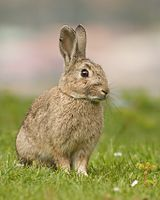
\includegraphics[height=2cm]{img/Oryctolagus_cuniculus_Tasmania_2.jpg}\\ 
 Fuchs & Hase 
\end{tabular}
\end{center}
\begin{flushright}
 in einem großen Wald
\end{flushright}
\scriptsize{sources:\\}
\scriptsize{https://en.wikipedia.org/wiki/File:Oryctolagus\_cuniculus\_Tasmania\_2.jpg}
\scriptsize{https://en.wikipedia.org/wiki/File:Vulpes\_vulpes\_laying\_in\_snow.jpg}

}


\frame
{
  \frametitle{Volterra-Lotka Model}
\begin{eqnarray}
 \dot u &=& \phantom{-} r u - p u v\nonumber\\
 \dot v &=& - s v + q u v \nonumber
\end{eqnarray}
Beute $u(t)$ und Räuber $v(t)$\newline\newline

ru:\\
Es gibt keine Räuber $\Rightarrow$ Anzahl der Beutetiere wächst exponentiell.\\
-puv:\\
Anzahl der gefressenen Beutetiere ist proportional zur Anzahl der Beutetiere und der Räuber\\
-sv:\\
Es gibt keine Beute $\Rightarrow$ Anzahl der Räuber fällt exponentiell.\\
quv:\\
Die Räuber beginnen sich zu vermehren, wenn Beute vorhanden ist.
}

\section{stationäre Punkte}
\frame
{
  \frametitle{Phasenraum}
Da $u(t), v(t)$ Populationen beschreiben, sind die stets positiv.\newline\newline
Phasengeschwindigkeit $F\left(u,v\right)$:
\begin{equation}
 \binom{\dot u}{\dot v} = F\left(u,v\right)= \binom{\phantom{-} r u - p u v}{- s v + q u v}\nonumber
\end{equation}\newline
\textcolor{blue} {Gibt es stationäre Punkte?}\\
\textcolor{blue} {Wie sieht das Vektorfeld der Phasengeschwindigkeit aus?}
}

\frame
{
  \frametitle{Phasenraum}
\textcolor{blue} {Gibt es stationäre Punkte?}\\
$\dot u=0,\dot v=0$\quad\quad$u_s= 0,v_s=0$ und $u_s= \frac{s}{q},v_s=\frac{r}{p}$\newline\newline
\textcolor{blue} {Wie sieht das Vektorfeld der Phasengeschwindigkeit aus?}
\begin{equation}
 F\left(u,v\right)= \binom{p u\left(v_s-v \right)}{q v\left(-u_s+u \right)}\nonumber
\end{equation}
%\begin{equation}
% F\left(x_s,y\right)= \binom{a x_s\left(y_s-y \right)}{0}\quad F\left(x,y_s\right)= \binom{0}{b y_s\left(-x_s+x \right)}\nonumber
%\end{equation}
\begin{center}
 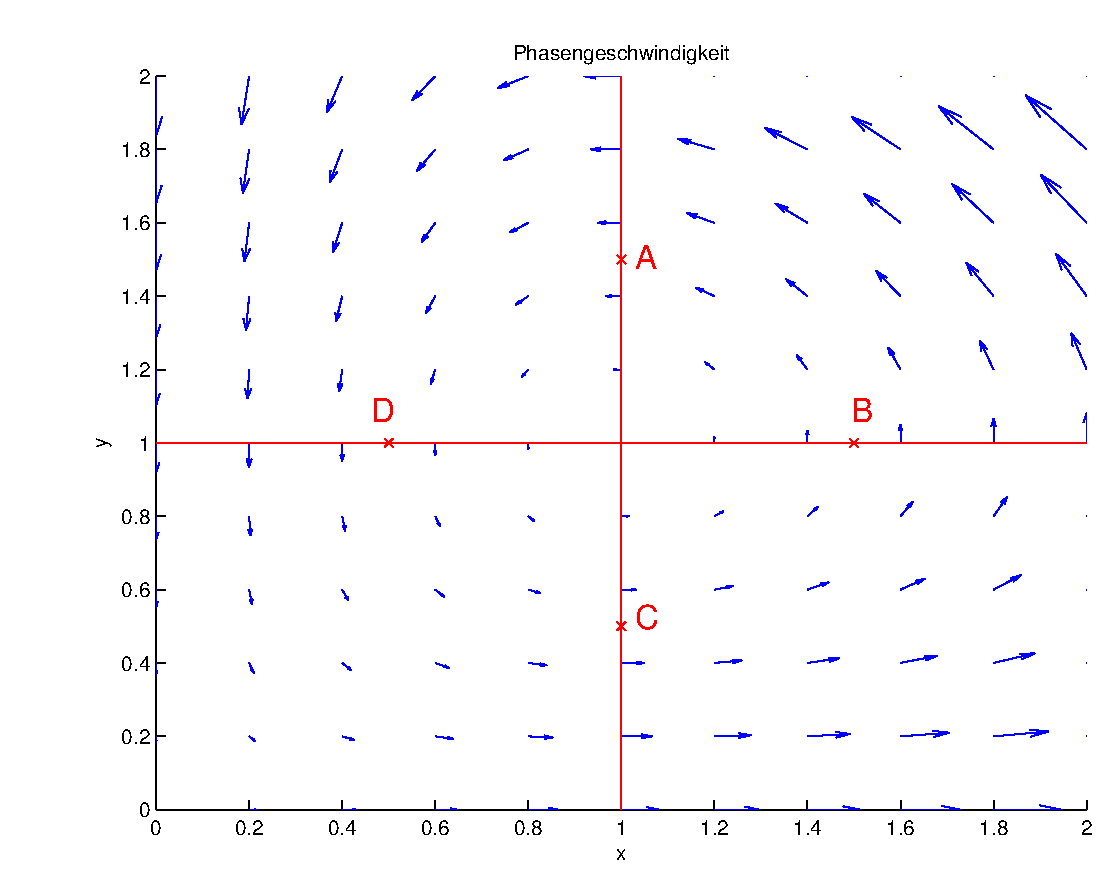
\includegraphics[scale=0.3]{img/Vektorfeld-eps-converted-to.pdf}
 \end{center}
}

\frame
{
  \frametitle{systematische Betrachtung der Fixpunkte}
  \textcolor{blue} {Welcher Art sind die Fixpunkte?}
\begin{equation}
 \dot u = f_1(u(t),v(t))\quad \dot v = f_2(u(t),v(t)) \nonumber
\end{equation}
 Linearisierung an dieser Stelle:
\begin{flushright}
\begin{tabular}{ll}
Jacobi-Matrix  & $J(u,v)=\begin{pmatrix} \frac{\partial f_1}{\partial u} & \frac{\partial f_1}{\partial v} \\ \frac{\partial f_2}{\partial u} & \frac{\partial f_2}{\partial v} \end{pmatrix}$
\end{tabular}
\end{flushright}
Die Eigenwerte von $J(u_s,v_s)$ seien $\lambda_{1},\lambda_{2}$.
\begin{tabular}{|l|ll|l|}\hline
$\lambda_{1},\lambda_{2} \in \mathbbm R$& $\lambda_{1}\lambda_{2}>0$ & $\lambda_{1},\lambda_{2} <0$& stabiler Knoten\\
& & $\lambda_{1},\lambda_{2} >0$& instabiler Knoten\\
& $\lambda_{1}\lambda_{2}<0$ & & Sattelpunkt\\\hline
$\lambda_{1,2} = \alpha \pm {\rm i} \beta$ & $\alpha<0$ & &stabiler Strudel\\
& $\alpha>0$ & & instabiler Strudel\\
& $\alpha=0$ & & Zentrum\\ \hline
\end{tabular}
}

\frame
{
  \frametitle{systematische Betrachtung der Fixpunkte}
  \textcolor{blue} {Welcher Art sind die Fixpunkte?}
\begin{equation}
 \dot u = f_1(u(t),v(t))=r u - p u v\quad \dot v = f_2(u(t),v(t))=- s v + q u v \nonumber
\end{equation}\newline\newline
\begin{tabular}{ll}
Jacobi-Matrix  & $J(u,v)=\begin{pmatrix} r -p v & - p u \\ q v & - s + q u \end{pmatrix}$
\end{tabular}\newline\newline\newline
$u_s= 0, v_s=0 \quad \Rightarrow \lambda_{1}=r,\lambda_{2}=-s \Rightarrow$ Sattelpunkt\newline\newline
$u_s= \frac{s}{q},v_s=\frac{r}{p} \quad \Rightarrow \lambda_{1}=i s r, \lambda_{2}=-i s r \Rightarrow$ Zentrum
}


\section{Verfahren}

\section{Algorithmen}
\frame
{
  \frametitle{Euler-Verfahren}
Anfangswertproblem:
\begin{equation}
 \dot y = f\left(t,y\right)\quad y\left(t_0\right)=y_0\nonumber
\end{equation}
Diskretisierung der Zeit:
\begin{equation}
 t_n = t_0 + n h \quad n=0,1,2,\cdots\nonumber
\end{equation}
Iteration der Lösung:
\begin{equation}
 y_{n+1} = y_n + h f \left(t_n,y_n\right)\nonumber
\end{equation}
}

\frame
{
  \frametitle{Runge-Kutta-Verfahren (vier Stufen)}
\begin{equation}
 \dot y = f\left(t,y\right)\quad y\left(t_0\right)=y_0\quad\quad t_n = t_0 + n h \quad n=0,1,2,\cdots\nonumber
\end{equation}
Iteration der Lösung:
\begin{eqnarray}
 y_{n+1} &=& y_n + h \left(\frac{1}{6} k_1+\frac{1}{3} k_2+\frac{1}{3} k_3+\frac{1}{6} k_4\right)\nonumber\\
 k_1 &=& f \left(t_n,y_n\right)\nonumber\\
 k_2 &=& f \left(t_n+\frac{h}{2},y_n+\frac{h}{2} k_1\right)\nonumber\\
 k_3 &=& f \left(t_n+\frac{h}{2},y_n+\frac{h}{2} k_2\right)\nonumber\\
 k_4 &=& f \left(t_n+h,y_n+h k_3\right)\nonumber
\end{eqnarray}
}

\frame
{
  \frametitle{Runge-Kutta-Verfahren (Allgemein)}
\begin{equation}
 \dot y = f\left(t,y\right)\quad y\left(t_0\right)=y_0\quad\quad t_k = t_0 + k h \quad k=0,1,2,\cdots\nonumber
\end{equation}

Iteration der Lösung:
\begin{equation}
 y_{k+1} = y_k + h \sum_{j=1}^s  b_j k_j\quad\quad k_j = f \left(t_k+h c_j,\,y_k+h \sum_{l=1}^s  a_{jl} k_l\right)\nonumber
\end{equation}

\begin{tabular}{lllll}
Tableau: & &Euler & & Runge-Kutta\\
\begin{tabular}{c|ccc}
$c_1$ & $a_{11}$ & $\cdots$ & $a_{1s}$\\
$\vdots$ & $\vdots$ &  & $\vdots$\\
$c_s$ & $a_{s1}$ & $\cdots$ & $a_{ss}$\\\hline
 & $b_1$ & $\ldots$ & $b_s$
\end{tabular}
 & \hspace{4cm}&
\begin{tabular}{c|c}
$0$ &  \\\hline
 & $1$ 
\end{tabular}
 & \hspace{4cm}&
\begin{tabular}{c|cccc}
$0$ &  &  & &\\
$\frac{1}{2}$ & $\frac{1}{2}$ &  & &\\
$\frac{1}{2}$ & $0$ & $\frac{1}{2}$ & &\\
$1$ & $0$ & $0$ & $1$&\\\hline
 & $\frac{1}{6}$ & $\frac{1}{3}$ & $\frac{1}{3}$& $\frac{1}{6}$
\end{tabular}
\end{tabular}
}




\end{document}
